\title{Warm-Up for February 18th, 2022}
\author{Dr. Jordan Hanson - Whittier College Dept. of Physics and Astronomy}
\date{\today}
\documentclass[12pt]{article}
\usepackage[a4paper, total={18cm, 27cm}]{geometry}
\usepackage{graphicx}
\usepackage{amsmath}
\usepackage{bm}
\begin{document}
\maketitle

\section{Electrostatics}

\begin{enumerate}
\item Find the electric field at a distance $z$ above the midpoint of a straight line segment of length $2L$ that carries a uniform line charge $\lambda$ (Fig. \ref{fig:line}
\begin{figure}[ht]
\centering
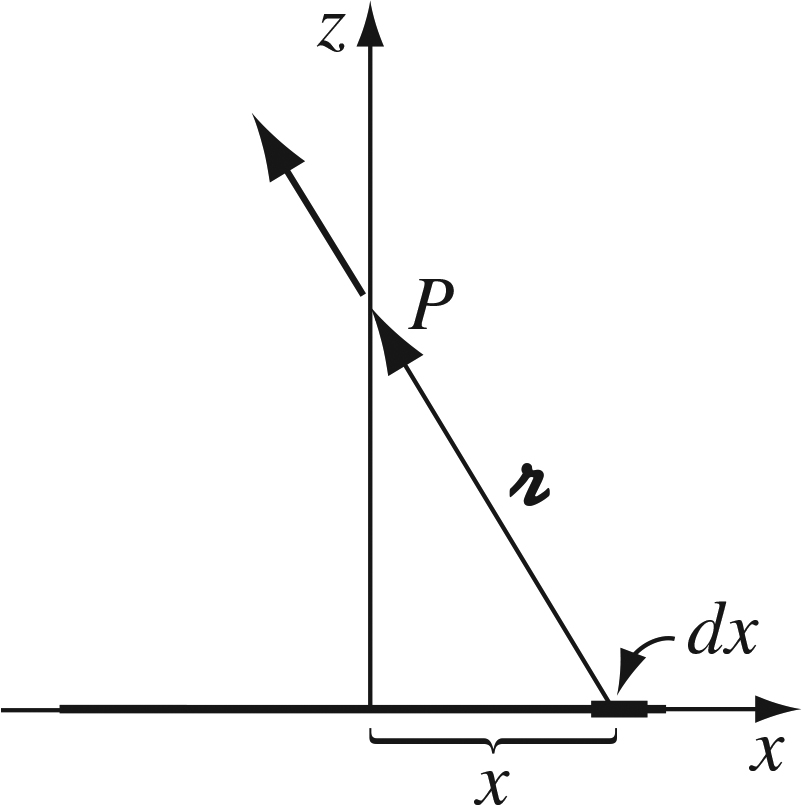
\includegraphics[width=0.33\textwidth]{figures/2_6.jpg}
\caption{\label{fig:line} A line of continuous, positive charge.}
\end{figure}
\item Re-work exercise 1, if the right side of the line is negative charge.  How does this field compare to the dipole system in the far-field limit?
\end{enumerate}

\end{document}